\documentclass{standalone}
\usepackage{tikz}
\usetikzlibrary{patterns, positioning}


\begin{document}
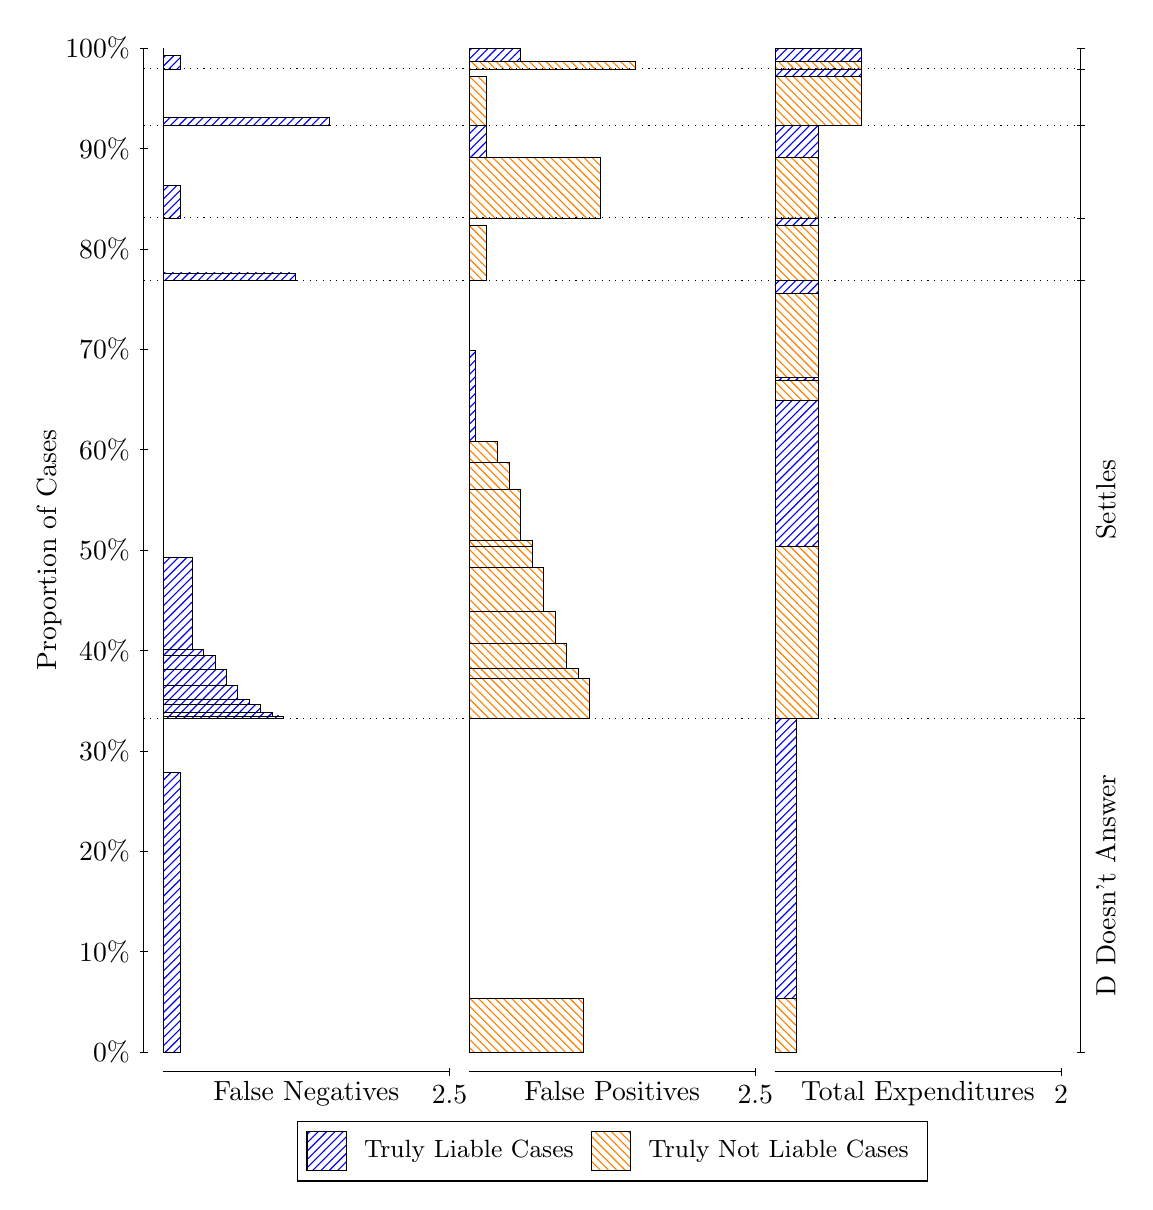
\begin{tikzpicture}
\draw[black, very thin] (1.5,1.75) -- (1.5,14.5);
\node[rotate=90, text=black, anchor=center] at (0.3, 8.125) {Proportion of Cases};
\draw[black, very thin] (1.45,1.75) -- (1.55,1.75);
\node[text=black, anchor=east] at (1.45, 1.75) {0\%};
\draw[black, very thin] (1.45,3.025) -- (1.55,3.025);
\node[text=black, anchor=east] at (1.45, 3.025) {10\%};
\draw[black, very thin] (1.45,4.3) -- (1.55,4.3);
\node[text=black, anchor=east] at (1.45, 4.3) {20\%};
\draw[black, very thin] (1.45,5.575) -- (1.55,5.575);
\node[text=black, anchor=east] at (1.45, 5.575) {30\%};
\draw[black, very thin] (1.45,6.85) -- (1.55,6.85);
\node[text=black, anchor=east] at (1.45, 6.85) {40\%};
\draw[black, very thin] (1.45,8.125) -- (1.55,8.125);
\node[text=black, anchor=east] at (1.45, 8.125) {50\%};
\draw[black, very thin] (1.45,9.4) -- (1.55,9.4);
\node[text=black, anchor=east] at (1.45, 9.4) {60\%};
\draw[black, very thin] (1.45,10.675) -- (1.55,10.675);
\node[text=black, anchor=east] at (1.45, 10.675) {70\%};
\draw[black, very thin] (1.45,11.95) -- (1.55,11.95);
\node[text=black, anchor=east] at (1.45, 11.95) {80\%};
\draw[black, very thin] (1.45,13.225) -- (1.55,13.225);
\node[text=black, anchor=east] at (1.45, 13.225) {90\%};
\draw[black, very thin] (1.45,14.5) -- (1.55,14.5);
\node[text=black, anchor=east] at (1.45, 14.5) {100\%};

\draw[black, very thin] (13.4,1.75) -- (13.4,14.5);
\draw[black, very thin] (13.35,1.75) -- (13.45,1.75);
\node[anchor=west] at (13.35, 1.75) {};
\draw[black, very thin] (13.35,5.9851) -- (13.45,5.9851);
\node[anchor=west] at (13.35, 5.9851) {};
\draw[black, very thin] (13.35,11.545) -- (13.45,11.545);
\node[anchor=west] at (13.35, 11.545) {};
\draw[black, very thin] (13.35,12.344) -- (13.45,12.344);
\node[anchor=west] at (13.35, 12.344) {};
\draw[black, very thin] (13.35,13.516) -- (13.45,13.516);
\node[anchor=west] at (13.35, 13.516) {};
\draw[black, very thin] (13.35,14.236) -- (13.45,14.236);
\node[anchor=west] at (13.35, 14.236) {};
\draw[black, very thin] (13.35,14.5) -- (13.45,14.5);
\node[anchor=west] at (13.35, 14.5) {};

\draw[black, very thin, pattern color=blue, pattern=north east lines] (1.75,1.75) rectangle (1.968,5.3056);
\draw[black, very thin, pattern color=orange, pattern=north west lines] (1.75,5.3056) rectangle (1.75,5.9851);
\draw[black, very thin, pattern color=blue, pattern=north east lines] (1.75,5.9851) rectangle (3.276,6.0182);
\draw[black, very thin, pattern color=blue, pattern=north east lines] (1.75,6.0182) rectangle (3.1307,6.0666);
\draw[black, very thin, pattern color=blue, pattern=north east lines] (1.75,6.0666) rectangle (2.9853,6.1682);
\draw[black, very thin, pattern color=blue, pattern=north east lines] (1.75,6.1682) rectangle (2.84,6.23);
\draw[black, very thin, pattern color=blue, pattern=north east lines] (1.75,6.23) rectangle (2.6947,6.404);
\draw[black, very thin, pattern color=blue, pattern=north east lines] (1.75,6.404) rectangle (2.5493,6.6063);
\draw[black, very thin, pattern color=blue, pattern=north east lines] (1.75,6.6063) rectangle (2.404,6.789);
\draw[black, very thin, pattern color=blue, pattern=north east lines] (1.75,6.789) rectangle (2.2587,6.8676);
\draw[black, very thin, pattern color=blue, pattern=north east lines] (1.75,6.8676) rectangle (2.1133,8.0297);
\draw[black, very thin, pattern color=orange, pattern=north west lines] (1.75,8.0297) rectangle (1.75,11.545);
\draw[black, very thin, pattern color=blue, pattern=north east lines] (1.75,11.545) rectangle (3.4213,11.644);
\draw[black, very thin, pattern color=orange, pattern=north west lines] (1.75,11.644) rectangle (1.75,12.344);
\draw[black, very thin, pattern color=blue, pattern=north east lines] (1.75,12.344) rectangle (1.968,12.752);
\draw[black, very thin, pattern color=orange, pattern=north west lines] (1.75,12.752) rectangle (1.75,13.516);
\draw[black, very thin, pattern color=blue, pattern=north east lines] (1.75,13.516) rectangle (3.8573,13.615);
\draw[black, very thin, pattern color=orange, pattern=north west lines] (1.75,13.615) rectangle (1.75,14.236);
\draw[black, very thin, pattern color=blue, pattern=north east lines] (1.75,14.236) rectangle (1.968,14.404);
\draw[black, very thin, pattern color=orange, pattern=north west lines] (1.75,14.404) rectangle (1.75,14.5);
\draw[black, very thin, pattern color=orange, pattern=north west lines] (5.6333,1.75) rectangle (7.0867,2.4294);
\draw[black, very thin, pattern color=blue, pattern=north east lines] (5.6333,2.4294) rectangle (5.6333,5.9851);
\draw[black, very thin, pattern color=orange, pattern=north west lines] (5.6333,5.9851) rectangle (7.1593,6.4931);
\draw[black, very thin, pattern color=orange, pattern=north west lines] (5.6333,6.4931) rectangle (7.014,6.6206);
\draw[black, very thin, pattern color=orange, pattern=north west lines] (5.6333,6.6206) rectangle (6.8687,6.9415);
\draw[black, very thin, pattern color=orange, pattern=north west lines] (5.6333,6.9415) rectangle (6.7233,7.3457);
\draw[black, very thin, pattern color=orange, pattern=north west lines] (5.6333,7.3457) rectangle (6.578,7.9059);
\draw[black, very thin, pattern color=orange, pattern=north west lines] (5.6333,7.9059) rectangle (6.4327,8.1771);
\draw[black, very thin, pattern color=orange, pattern=north west lines] (5.6333,8.1771) rectangle (6.4327,8.2488);
\draw[black, very thin, pattern color=orange, pattern=north west lines] (5.6333,8.2488) rectangle (6.2873,8.8957);
\draw[black, very thin, pattern color=orange, pattern=north west lines] (5.6333,8.8957) rectangle (6.142,9.2391);
\draw[black, very thin, pattern color=orange, pattern=north west lines] (5.6333,9.2391) rectangle (5.9967,9.5006);
\draw[black, very thin, pattern color=blue, pattern=north east lines] (5.6333,9.5006) rectangle (5.706,10.663);
\draw[black, very thin, pattern color=blue, pattern=north east lines] (5.6333,10.663) rectangle (5.6333,11.545);
\draw[black, very thin, pattern color=orange, pattern=north west lines] (5.6333,11.545) rectangle (5.8513,12.245);
\draw[black, very thin, pattern color=blue, pattern=north east lines] (5.6333,12.245) rectangle (5.6333,12.344);
\draw[black, very thin, pattern color=orange, pattern=north west lines] (5.6333,12.344) rectangle (7.3047,13.108);
\draw[black, very thin, pattern color=blue, pattern=north east lines] (5.6333,13.108) rectangle (5.8513,13.516);
\draw[black, very thin, pattern color=orange, pattern=north west lines] (5.6333,13.516) rectangle (5.8513,14.137);
\draw[black, very thin, pattern color=blue, pattern=north east lines] (5.6333,14.137) rectangle (5.6333,14.236);
\draw[black, very thin, pattern color=orange, pattern=north west lines] (5.6333,14.236) rectangle (7.7407,14.332);
\draw[black, very thin, pattern color=blue, pattern=north east lines] (5.6333,14.332) rectangle (6.2873,14.5);
\draw[black, very thin, pattern color=orange, pattern=north west lines] (9.5167,1.75) rectangle (9.7892,2.4294);
\draw[black, very thin, pattern color=blue, pattern=north east lines] (9.5167,2.4294) rectangle (9.7892,5.9851);
\draw[black, very thin, pattern color=orange, pattern=north west lines] (9.5167,5.9851) rectangle (10.062,8.1771);
\draw[black, very thin, pattern color=blue, pattern=north east lines] (9.5167,8.1771) rectangle (10.062,10.024);
\draw[black, very thin, pattern color=orange, pattern=north west lines] (9.5167,10.024) rectangle (10.062,10.285);
\draw[black, very thin, pattern color=blue, pattern=north east lines] (9.5167,10.285) rectangle (10.062,10.319);
\draw[black, very thin, pattern color=orange, pattern=north west lines] (9.5167,10.319) rectangle (10.062,11.381);
\draw[black, very thin, pattern color=blue, pattern=north east lines] (9.5167,11.381) rectangle (10.062,11.545);
\draw[black, very thin, pattern color=orange, pattern=north west lines] (9.5167,11.545) rectangle (10.062,12.245);
\draw[black, very thin, pattern color=blue, pattern=north east lines] (9.5167,12.245) rectangle (10.062,12.344);
\draw[black, very thin, pattern color=orange, pattern=north west lines] (9.5167,12.344) rectangle (10.062,13.108);
\draw[black, very thin, pattern color=blue, pattern=north east lines] (9.5167,13.108) rectangle (10.062,13.516);
\draw[black, very thin, pattern color=orange, pattern=north west lines] (9.5167,13.516) rectangle (10.607,14.137);
\draw[black, very thin, pattern color=blue, pattern=north east lines] (9.5167,14.137) rectangle (10.607,14.236);
\draw[black, very thin, pattern color=orange, pattern=north west lines] (9.5167,14.236) rectangle (10.607,14.332);
\draw[black, very thin, pattern color=blue, pattern=north east lines] (9.5167,14.332) rectangle (10.607,14.5);
\draw[black, dotted] (1.5,5.9851) -- (13.4,5.9851);
\draw[black, dotted] (1.5,11.545) -- (13.4,11.545);
\draw[black, dotted] (1.5,12.344) -- (13.4,12.344);
\draw[black, dotted] (1.5,13.516) -- (13.4,13.516);
\draw[black, dotted] (1.5,14.236) -- (13.4,14.236);
\draw[black, very thin] (1.75,1.5) -- (5.3833,1.5);
\node[text=black, anchor=north] at (3.5667, 1.5) {False Negatives};
\draw[black, very thin] (5.3833,1.45) -- (5.3833,1.55);
\node[text=black, anchor=north] at (5.3833, 1.45) {2.5};

\draw[black, very thin] (5.6333,1.5) -- (9.2667,1.5);
\node[text=black, anchor=north] at (7.45, 1.5) {False Positives};
\draw[black, very thin] (9.2667,1.45) -- (9.2667,1.55);
\node[text=black, anchor=north] at (9.2667, 1.45) {2.5};

\draw[black, very thin] (9.5167,1.5) -- (13.15,1.5);
\node[text=black, anchor=north] at (11.333, 1.5) {Total Expenditures};
\draw[black, very thin] (13.15,1.45) -- (13.15,1.55);
\node[text=black, anchor=north] at (13.15, 1.45) {2};

\node[text=black, centered, rotate=90] at (13.72, 3.8675) {D Doesn't Answer};
\node[text=black, centered, rotate=90] at (13.72, 8.7652) {Settles};





\draw (7.449999999999999,1.5) node[draw=none] (baseCoordinate) {};
\begin{scope}[align=center]
        \matrix[scale=0.5, draw=black, below=0.5cm of baseCoordinate, nodes={draw}, column sep=0.1cm]{
            \node[rectangle, draw, minimum width=0.5cm, minimum height=0.5cm, pattern color=blue, pattern=north east lines] {}; &
            \node[draw=none, font=\small, text=black] (B) {Truly Liable Cases}; &
            \node[rectangle, draw, minimum width=0.5cm, minimum height=0.5cm, pattern color=orange, pattern=north west lines] {}; &
            \node[draw=none, font=\small, text=black] (B) {Truly Not Liable Cases}; \\
            };
\end{scope}

\end{tikzpicture}
\end{document}